\documentclass[border=10pt]{standalone}
\usepackage[svgnames]{xcolor}
\usepackage{amsmath}
\usepackage{pgfplots}
\pgfplotsset{compat=newest}
\usepackage[sfdefault]{FiraSans}
\usepackage{FiraMono}
\renewcommand*\familydefault{\sfdefault}
\begin{document}
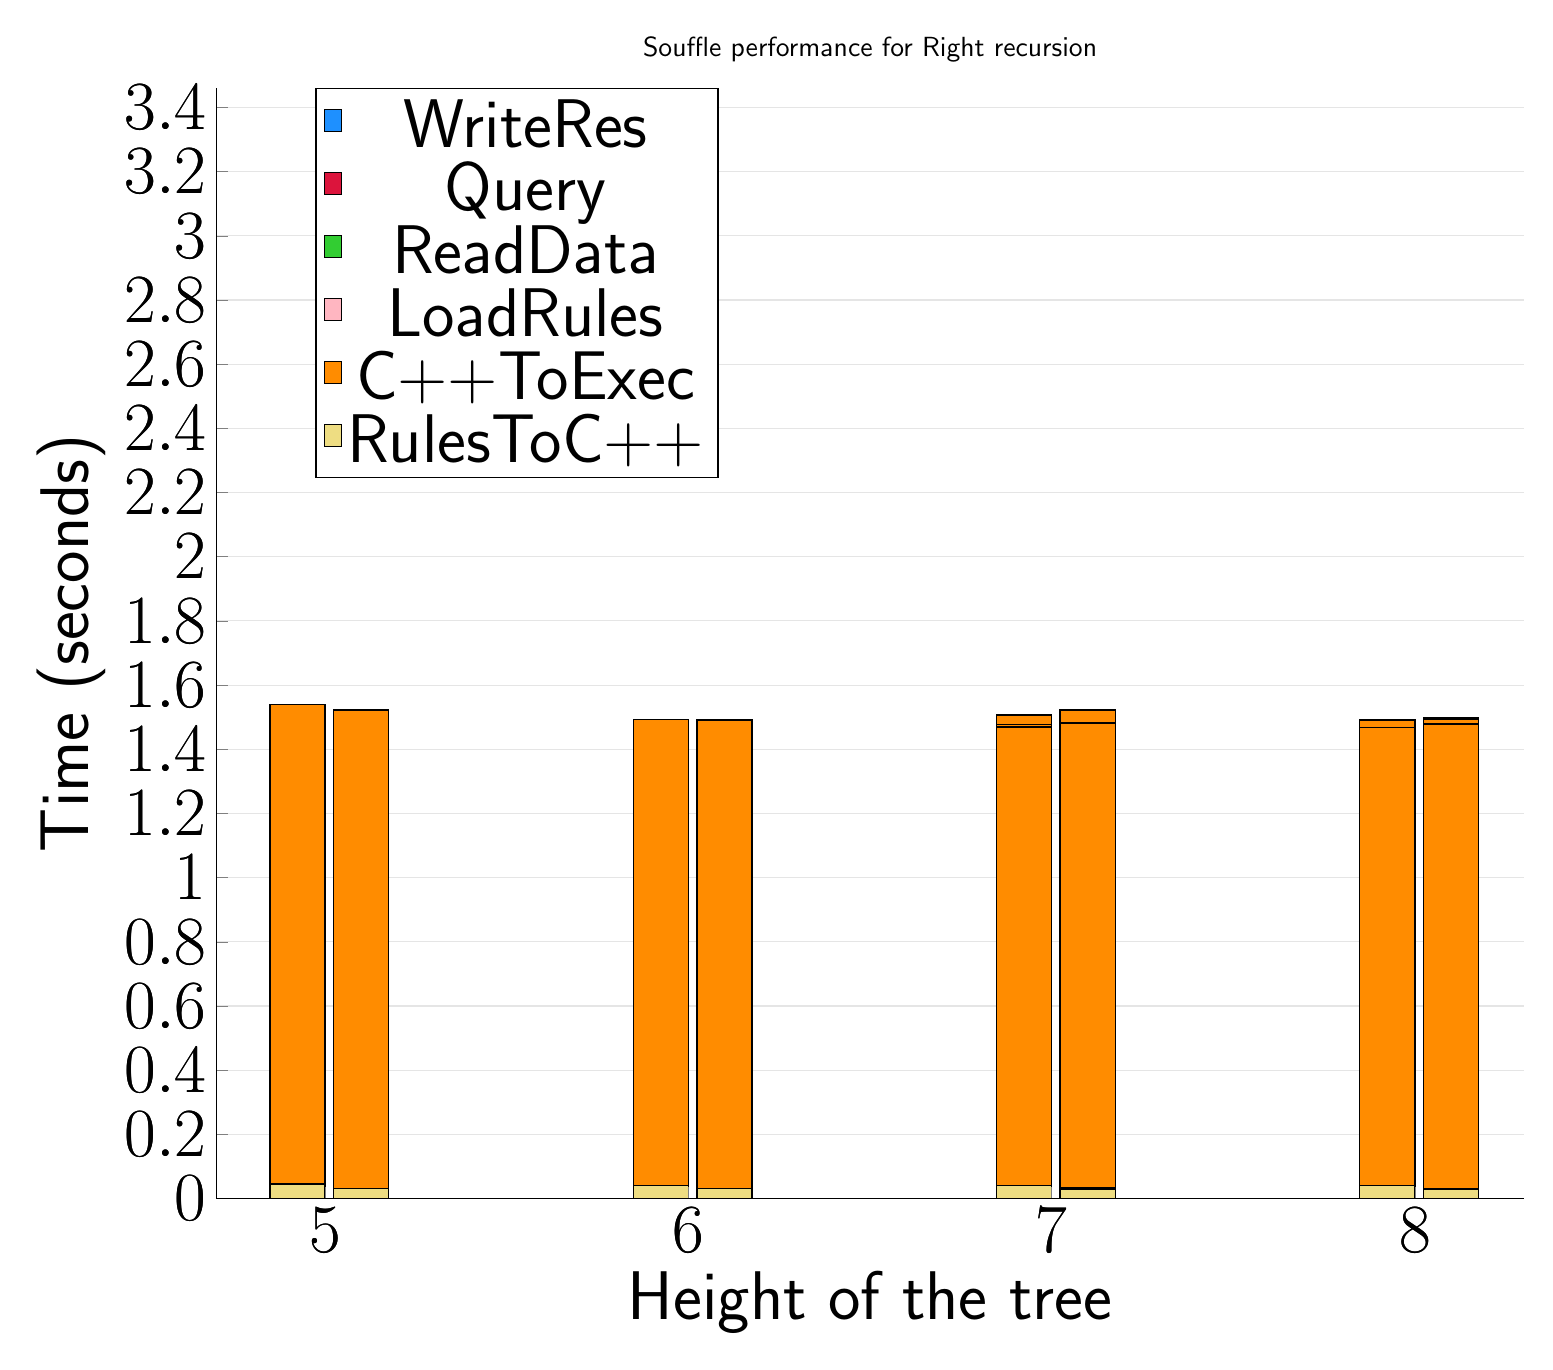
\begin{tikzpicture}
\begin{axis}[
   ybar stacked,
   title={Souffle performance for Right recursion},
   bar shift=-10pt,
   width=1.5\textwidth,
   bar width=0.7cm,
   ymajorgrids, tick align=inside,
   major grid style={draw=gray!20},
   xtick=data,
   ymin=0, ymax=3.4609999895095824,
   axis x line*=bottom,
   axis y line*=left,
   enlarge x limits=0.1,
   legend style={
       at={(0.23, 1)},
       anchor=north,
       legend columns=1,
       font=\Huge,
   },
   ylabel={Time (seconds)},
   xlabel={Height of the tree},
   label style={font=\Huge},
   tick label style={font=\Huge},
]
\addlegendimage{fill=DodgerBlue, draw=black, line width=0.2pt}
\addlegendentry{WriteRes}
\addlegendimage{fill=Crimson, draw=black, line width=0.2pt}
\addlegendentry{Query}
\addlegendimage{fill=LimeGreen, draw=black, line width=0.2pt}
\addlegendentry{ReadData}
\addlegendimage{fill=LightPink, draw=black, line width=0.2pt}
\addlegendentry{LoadRules}
\addlegendimage{fill=DarkOrange, draw=black, line width=0.2pt}
\addlegendentry{C++ToExec}
\addlegendimage{fill=LightGoldenrod, draw=black, line width=0.2pt}
\addlegendentry{RulesToC++}
\addplot +[fill=LightGoldenrod, draw=black, line width=0.5pt] coordinates {
    (5, 0.045999979972839354)
    (6, 0.040999984741210936)
    (7, 0.04000005722045898)
    (7, 0.04100003242492676)
    (7, 0.04000000953674317)
    (8, 0.04100003242492676)
    (8, 0.04000005722045898)
    (8, 0.039999985694885255)
};
\addplot +[fill=DarkOrange, draw=black, line width=0.5pt] coordinates {
    (5, 1.4930000066757203)
    (6, 1.4509999990463256)
    (7, 1.4369999647140503)
    (7, 1.4289999961853028)
    (7, 1.466000008583069)
    (8, 1.4259999990463257)
    (8, 1.4489999532699585)
    (8, 1.4270000219345094)
};
\addplot +[fill=LightPink, draw=black, line width=0.5pt] coordinates {
    (5, 1.32292e-05)
    (6, 0.0)
    (7, 0.0)
    (7, 0.0)
    (7, 0.0)
    (8, 0.0)
    (8, 1.1025e-05)
    (8, 0.0)
};
\addplot +[fill=LimeGreen, draw=black, line width=0.5pt] coordinates {
    (5, 0.00040792910000000005)
    (6, 0.00045705830000000003)
    (7, 0.0005525081999999999)
    (7, 0.0006413205000000001)
    (7, 0.0005235458000000001)
    (8, 0.0008530082999999999)
    (8, 0.0008011041999999999)
    (8, 0.0009817205000000001)
};
\addplot +[fill=Crimson, draw=black, line width=0.5pt] coordinates {
    (5, 0.0001487291)
    (6, 0.0003439)
    (7, 0.0007549459999999999)
    (7, 0.0008271002)
    (7, 0.0007063749)
    (8, 0.0019441709999999997)
    (8, 0.0017303280000000002)
    (8, 0.0019745540000000003)
};
\addplot +[fill=DodgerBlue, draw=black, line width=0.5pt] coordinates {
    (5, 0.0008191331000000001)
    (6, 0.000388283)
    (7, 0.0004594669)
    (7, 0.0007207130000000001)
    (7, 0.000522042)
    (8, 0.0009659834)
    (8, 0.0008564581999999999)
    (8, 0.0009590461)
};
\end{axis}
\begin{axis}[
   ybar stacked,
   bar shift=13pt,
   width=1.5\textwidth,
   bar width=0.7cm,
   ymajorgrids, tick align=inside,
   major grid style={draw=none},
   xtick=data,
   ymin=0, ymax=3.4609999895095824,
   axis x line*=none,
   axis y line*=none,
   enlarge x limits=0.1,
   label style={font=\Huge},
   tick label style={font=\Huge},
]
\addplot +[fill=LightGoldenrod, draw=black, line width=0.5pt] coordinates {
    (5, 0.031000000000000007)
    (6, 0.031000000000000007)
    (7, 0.030000000000000006)
    (7, 0.030000000000000006)
    (7, 0.032999999999999995)
    (8, 0.030000000000000006)
    (8, 0.030000000000000006)
    (8, 0.030000000000000006)
};
\addplot +[fill=DarkOrange, draw=black, line width=0.5pt] coordinates {
    (5, 1.492)
    (6, 1.4599999999999997)
    (7, 1.454)
    (7, 1.451)
    (7, 1.4880000000000002)
    (8, 1.4489999999999998)
    (8, 1.464)
    (8, 1.449)
};
\addplot +[fill=LightPink, draw=black, line width=0.5pt] coordinates {
    (5, 1.3100000000000002e-05)
    (6, 0.0)
    (7, 0.0)
    (7, 0.0)
    (7, 0.0)
    (8, 0.0)
    (8, 1.09e-05)
    (8, 0.0)
};
\addplot +[fill=LimeGreen, draw=black, line width=0.5pt] coordinates {
    (5, 0.00039299999999999996)
    (6, 0.00043950000000000006)
    (7, 0.0005379)
    (7, 0.0005786999999999999)
    (7, 0.0005075)
    (8, 0.0008423)
    (8, 0.0007861999999999999)
    (8, 0.0008617000000000002)
};
\addplot +[fill=Crimson, draw=black, line width=0.5pt] coordinates {
    (5, 0.00014810000000000002)
    (6, 0.00033820000000000003)
    (7, 0.0007549)
    (7, 0.0008265)
    (7, 0.0007059999999999999)
    (8, 0.0019427)
    (8, 0.00173)
    (8, 0.0019735000000000004)
};
\addplot +[fill=DodgerBlue, draw=black, line width=0.5pt] coordinates {
    (5, 0.0003039)
    (6, 0.00030809999999999995)
    (7, 0.0004587)
    (7, 0.0004944)
    (7, 0.00044610000000000006)
    (8, 0.0009054)
    (8, 0.0008553000000000001)
    (8, 0.0009327000000000001)
};
\end{axis}
\end{tikzpicture}

\end{document}
